\documentclass{sigchi}

% Use this command to override the default ACM copyright statement (e.g. for preprints). 
% Consult the conference website for the camera-ready copyright statement.


%% EXAMPLE BEGIN -- HOW TO OVERRIDE THE DEFAULT COPYRIGHT STRIP -- (July 22, 2013 - Paul Baumann)
 %\toappear{Permission to make digital or hard copies of all or part of this work for personal or classroom use is 	granted without fee provided that copies are not made or distributed for profit or commercial advantage and that copies bear this notice and the full citation on the first page. Copyrights for components of this work owned by others than ACM must be honored. Abstracting with credit is permitted. To copy otherwise, or republish, to post on servers or to redistribute to lists, requires prior specific permission and/or a fee. Request permissions from permissions@acm.org. \\
% {\emph{CHI'14}}, April 26--May 1, 2014, Toronto, Canada. \\
% Copyright \copyright~2014 ACM ISBN/14/04...\$15.00. \\
% DOI string from ACM form confirmation}
%% EXAMPLE END -- HOW TO OVERRIDE THE DEFAULT COPYRIGHT STRIP -- (July 22, 2013 - Paul Baumann)


% Arabic page numbers for submission. 
% Remove this line to eliminate page numbers for the camera ready copy
% \pagenumbering{arabic}


% Load basic packages
\usepackage{balance}  % to better equalize the last page
\usepackage{graphics} % for EPS, load graphicx instead
\usepackage{times}    % comment if you want LaTeX's default font
\usepackage{url}      % llt: nicely formatted URLs

% llt: Define a global style for URLs, rather that the default one
\makeatletter
\def\url@leostyle{%
  \@ifundefined{selectfont}{\def\UrlFont{\sf}}{\def\UrlFont{\small\bf\ttfamily}}}
\makeatother
\urlstyle{leo}


% To make various LaTeX processors do the right thing with page size.
\def\pprw{8.5in}
\def\pprh{11in}
\special{papersize=\pprw,\pprh}
\setlength{\paperwidth}{\pprw}
\setlength{\paperheight}{\pprh}
\setlength{\pdfpagewidth}{\pprw}
\setlength{\pdfpageheight}{\pprh}

% Make sure hyperref comes last of your loaded packages, 
% to give it a fighting chance of not being over-written, 
% since its job is to redefine many LaTeX commands.
\usepackage[pdftex]{hyperref}
\hypersetup{
pdftitle={SIGCHI Conference Proceedings Format},
pdfauthor={LaTeX},
pdfkeywords={SIGCHI, proceedings, archival format},
bookmarksnumbered,
pdfstartview={FitH},
colorlinks,
citecolor=black,
filecolor=black,
linkcolor=black,
urlcolor=black,
breaklinks=true,
}

% create a shortcut to typeset table headings
\newcommand\tabhead[1]{\small\textbf{#1}}


% End of preamble. Here it comes the document.
\begin{document}

\title{Controlling Rapid Serial Visual Presentation of Text with mobile EEG Devices}

\numberofauthors{4}
\author{
  \alignauthor Thomas Maillart\\
    \affaddr{UC Berkeley, School of Information}\\
    \affaddr{102 South Hall, Berkeley, CA 94720}\\
    \email{thomas.maillart@ischool.berkeley.edu}\\
    %\affaddr{Optional phone number}
  \alignauthor Nick Merrill\\
    \affaddr{UC Berkeley, School of Information}\\
    \affaddr{102 South Hall, Berkeley, CA 94720 }\\
   \email{ffff@berkeley.edu}\\
    %\affaddr{Optional phone number}    
  \alignauthor John Chuang\\
    \affaddr{UC Berkeley, School of Information}\\
    \affaddr{102 South Hall, Berkeley, CA 94720}\\
    \email{chuang@ischool.berkeley.edu}\\
    %\affaddr{Optional phone number}
    %\alignauthor Benjamin Johnson\\
    %\affaddr{UC Berkeley, School of Information}\\
    %\affaddr{102 South Hall, Berkeley, CA 94720}\\
    %\email{johnsonb@ischool.berkeley.edu}\\
    %\affaddr{Optional phone number}
}

\maketitle

\begin{abstract}
At the age of online information abundance, the human capacity to retain knowledge is largely limited by the time and the attention required to read text, watch videos, listen to podcasts. For written information, rapid serial visual presentation (RSVP) helps greatly save time with similar levels of text understanding, compared with traditional reading. However, RSVP does not account for attention. We present a simple hybrid brain-computer interface (BCI) that controls in real-time the speed of reading by measuring the instant level of higher cognitive brain activity. Electroencephalogram (EEG) signal is acquired with a single channel consumer-grade headset and analyzed in the frequency domain. The pace of word display is controlled by a measure brainwave entropy. We have conducted a controlled experiment with 50 subjects with three distinct treatments, and we show that brain-controlled speed-reading increases the speed and the understanding of texts by subjects.
\end{abstract}

\keywords{BCI, Entropy, Speed-Reading, Cognitive Attention}

\category{H.5.m.}{Information Interfaces and Presentation (e.g. HCI)}{Miscellaneous}


\section{Introduction}

\section{Related Work}

\subsection{RSVP}



\subsection{Brainwaves}





\section{Method}

\subsection{Brain Speed Reader}

{\bf describe the brain control system}

\begin{enumerate}
  \item capture brainwaves for 1 second
  \item compute power spectrum
  \item compute normalized entropy
  \item update display speed ({\bf trick of the moving average to be described here})
\end{enumerate}


\subsection{Experimental Protocol}


\begin{enumerate}
  \item Constant Rate
  %\item Randomly Varying Text : AR(1) $\rigtharrow$ AR1(n,baseline,baseline/2,0.5,sigma=std) AR1 formula : $c + phi * X[-1] + np.random.normal(scale=sigma)$
  %\item Brain Speed Reader : (i) compute entropy $S$ at t, (ii) normalize $S$ as $S_{norm} = (S- \langle S \rangle) / \sigma_S$, with $\langle S \rangle$ and $\sigma_S$ computed over the last XX values of entropy, (iii) compute a new speed as $v(t+1) = v(t)\cdot(1-0.2\sdot S_{norm})$
\end{enumerate}


\subsection{Measuring Text Complexity}

ATOS  ( ref: Michael Milone,The Development of ATOS, The Renaissance Readability Formula, p10 (2010) \url{http://doc.renlearn.com/KMNet/R004250827GJ11C4.pdf}

\begin{itemize}
  \item Words per sentence
  \item Average grade level of words ( which class grade the word is first seen)
  \item Characters per word
\end{itemize}


$ATOS Rasch Difficulty Formula = -8.54 + 1.95 * Ln(AvgWords) + .46 * AvgGrad100 + 1.74 * Ln(AvgChar)$

Adjustment for books with less than 500 words

$BLGL for Books With Fewer Than 500 Words = .004 * Book Length + 0.4$


Table detailing texts : \url{https://docs.google.com/spreadsheets/d/1uwkoToM-p3UFrd0U_1vOX4eBJsmYuPVYVhvhsZ8Y5Nc/edit#gid=0}




%\begin{itemize}
%  \item {\bf text 0 (adapted from Coming of Age in Samoa, Margaret Mead, 1928
%)}:   $ATOS=9.5$,  $word~count = 421$
%  \item {\bf Text 1  (adapted from The Warden, Anthony Trollope, 1855)} : $ATOS=8.3$, $word~count = 563$
%  \item {\bf Text 2  (adapted from The Mayor of Casterbridge, Thomas Hardy, 1886) } : $ATOS=10.2$, $word~count = 831$
%  \item {\bf Text 3 (Adapted from: The Social Function of Science, John D Bernal (1939))} : $ATOS=11.9$, $word~count = 421$
%\end{itemize}



\begin{figure}[!h]
\centering
%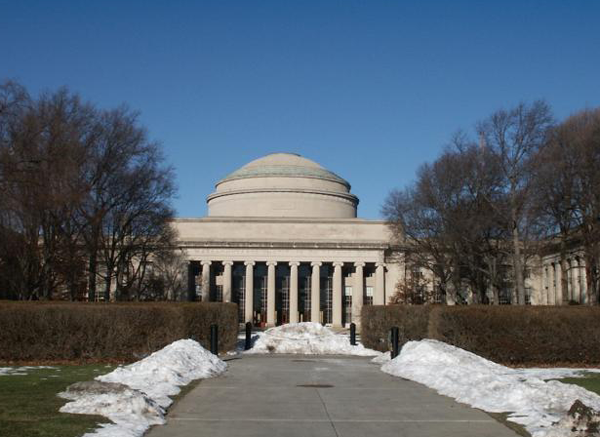
\includegraphics[width=0.9\columnwidth]{Figure1}
\caption{With Caption Below, be sure to have a good resolution image
  (see item D within the preparation instructions).}
\label{fig:figure1}
\end{figure}

\begin{table}
  \centering
  \begin{tabular}{|c|c|c|}
    \hline
    \tabhead{Objects} &
    \multicolumn{1}{|p{0.3\columnwidth}|}{\centering\tabhead{Caption --- pre-2002}} &
    \multicolumn{1}{|p{0.4\columnwidth}|}{\centering\tabhead{Caption --- 2003 and afterwards}} \\
    \hline
    Tables & Above & Below \\
    \hline
    Figures & Below & Below \\
    \hline
  \end{tabular}
  \caption{Table captions should be placed below the table.}
  \label{tab:table1}
\end{table}


\section{Acknowledgments}
T. Maillart acknowledges SNF Grant ....
\balance


\bibliographystyle{acm-sigchi}
\bibliography{sample}
\end{document}
